\section{Integrazione LoRa}

\begin{frame}[fragile]
  \frametitle{LoRaWAN Classes}
  \begin{figure}
    \centering
    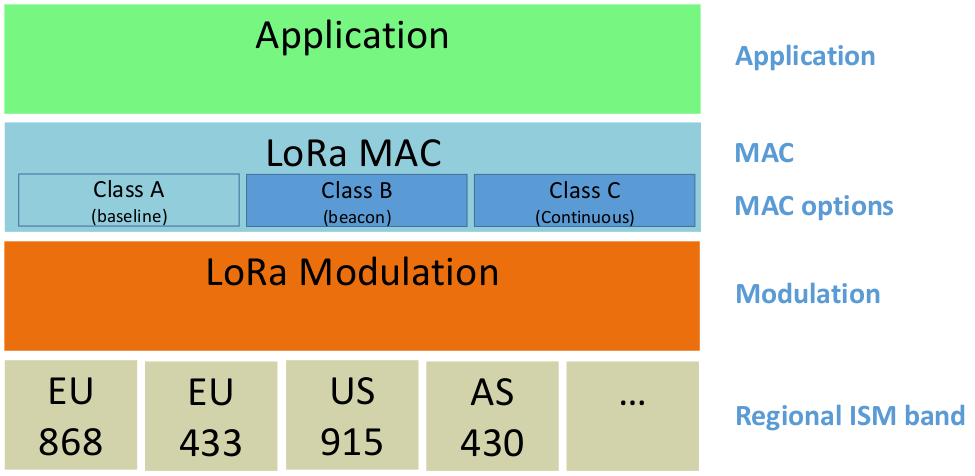
\includegraphics[width=0.9\textwidth]{img/loraClasses.png}
  \end{figure}
\end{frame}


\begin{frame}[fragile]
  \frametitle{Class A end-devices}
  \begin{itemize}
    \item Its funtionalities are implemented by every end-device.
    \item Uplink: devices transmit following Aloha method.
    \item Downlink: after a transmission two tiny time windows are opened to allow reception
    \begin{itemize}
      \item RX1 uses the same frequency channel as the uplink and a data rate depending on the one in the uplink;
      \item RX2 uses a fixed configurable frequency and data rate;
      \item Devices is active in rx only if a preamble is detected.
    \end{itemize}
  \end{itemize}
  \begin{figure}
		\centering
		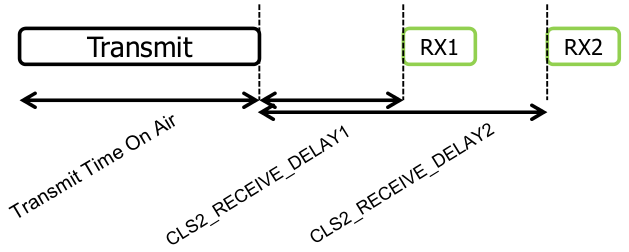
\includegraphics[width=0.4\textwidth]{img/lora_rx_windows.png}
  \end{figure}
\end{frame}

\begin{frame}[fragile]
  \frametitle{Class B end-devices}
  \begin{itemize}
		\item Class B end-devices are optimized for mobile and fixed battery-powered end-devices.
		\item They add a synchronized reception window called ``ping slot''
		\begin{itemize}
			\item Synchronization requires beacons;
			\item Devices selects randomly a ping slot at each beacon to avoid collisions.
		\end{itemize}
	\end{itemize}
	\begin{figure}
		\centering
		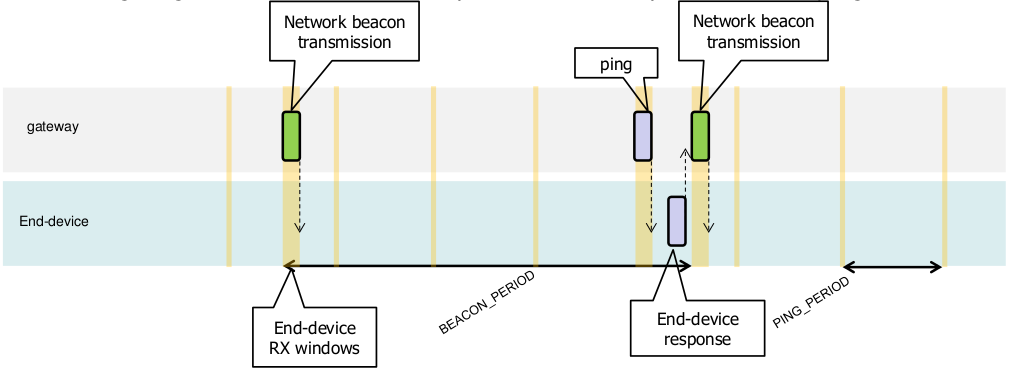
\includegraphics[width=0.8\textwidth]{img/loraBeacon.png}
	\end{figure}
\end{frame}

\begin{frame}[fragile]
  \frametitle{Class B end-devices}
  \begin{itemize}
		\item All end-devices start and join the network as end-devices of Class A.
		\item The end-device application can then decide to switch to Class B.
		\item The end-device waits a beacon and selects a ping slot of 30 ms from the 4096 available in a beacon interval.
		\item When the mote is far from BS the duration is extended, if beacon is not received the device tries to mantain the synchronization for 2 hours after that it returns to class A
  \end{itemize}
\end{frame}

\begin{frame}[fragile]
	\frametitle{Class C end-devices}
	\begin{itemize}
		\item This mode is used when there are no need for energy awareness and there's no need to minimize reception time.
		\item Class C end-devices cannot implement Class B option.
		\item These devices will listen with RX2 windows parameters as often as possible.
	\end{itemize}
	\begin{figure}
		\centering
		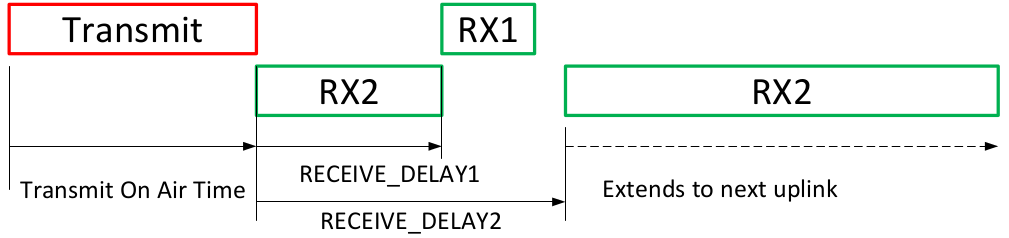
\includegraphics[width=0.8\textwidth]{img/loraClassC.png}
	\end{figure}
\end{frame}
